\chapter{Event Reconstruction}
\label{chapter:eventReco}

The data (and the Monte Carlo simulations) come out of the detector (or its
emulated counterpart) in similar collections of raw measurements. At this stage,
only information about tracker hits, muon chamber hits, and calorimeter deposits
exist. In order to be useful in a physics setting, these detector signatures must be
translated into their physics counterparts. The process of running the raw data
through complex algorithms designed to pick out the myriad particles in the
event is called \emph{reconstruction.} A full description of the reconstruction
algorithms utilized in this analysis follows.

\section{Vertex and Track Reconstruction}
The first step in reconstructing the physics content of an event is mapping
hits in the silicon tracker systems to a particle. This is done using a
\emph{Kalman Filter,} which starts at an inner tracking `seed' point and adds
successive hits to each potential track. As it adds hits to the potential
tracks, it propagates a likely position for a next hit forward, giving the
algorithm a place to look for the next contribution. After the track is built,
the process is repeated, building a track from the outermost hits to the inner
regions. This has the effect of smoothing the overall track and minimizing the
measuring errors at the vertex origin~\cite{trackBuilding}. 

Because each event is accompanied by a large number of pile-up events (up to 35
in 2012 running),  it is important to be able to distinguish each particles'
tracks along with where, with respect to the interaction point, they originated
from. These places of origin, known as vertices, are reconstructed in two
phases. First is the \emph{track finding} algorithms, which associate the
measured tracks with a potential vertex. This is done via \emph{deterministic
annealing}, a machine learning algorithm which models the tracks as a
thermodynamic system, clustering the tracks by minimizing the effective free
energy of the system~\cite{detAnnealing, cmsdetAnnealing}. Vertex fitting, on
the other hand, is the process of measuring a vertex's properties (especially
its position and associated errors). Once a vertex is found and fit, the tracks
are again recalculated, using the vertex as an additional position in the track
fit algorithm~\cite{vertexFitting}. In order to separate the vertices associated
with pileup events with the interaction of interest, each event is given a
\emph{primary vertex,} defined to be the one with the highest sum of squared
track transverse momenta.

\section{Electron Reconstruction} 
Electron reconstruction at CMS comprises of combining tracks with matching
\emph{superclusters}, large groups of associated clusters in the ECAL (see
Fig.~\ref{fig:eleReco}). In supercluster construction, the smaller clusters are
collected in such a way as to capture both the primary ECAL deposit and the
deposits spread in $\phi$ that result from bremsstrahlung radiation as the
electron travels its helical course through the detector.

\begin{figure}[h]
\centering
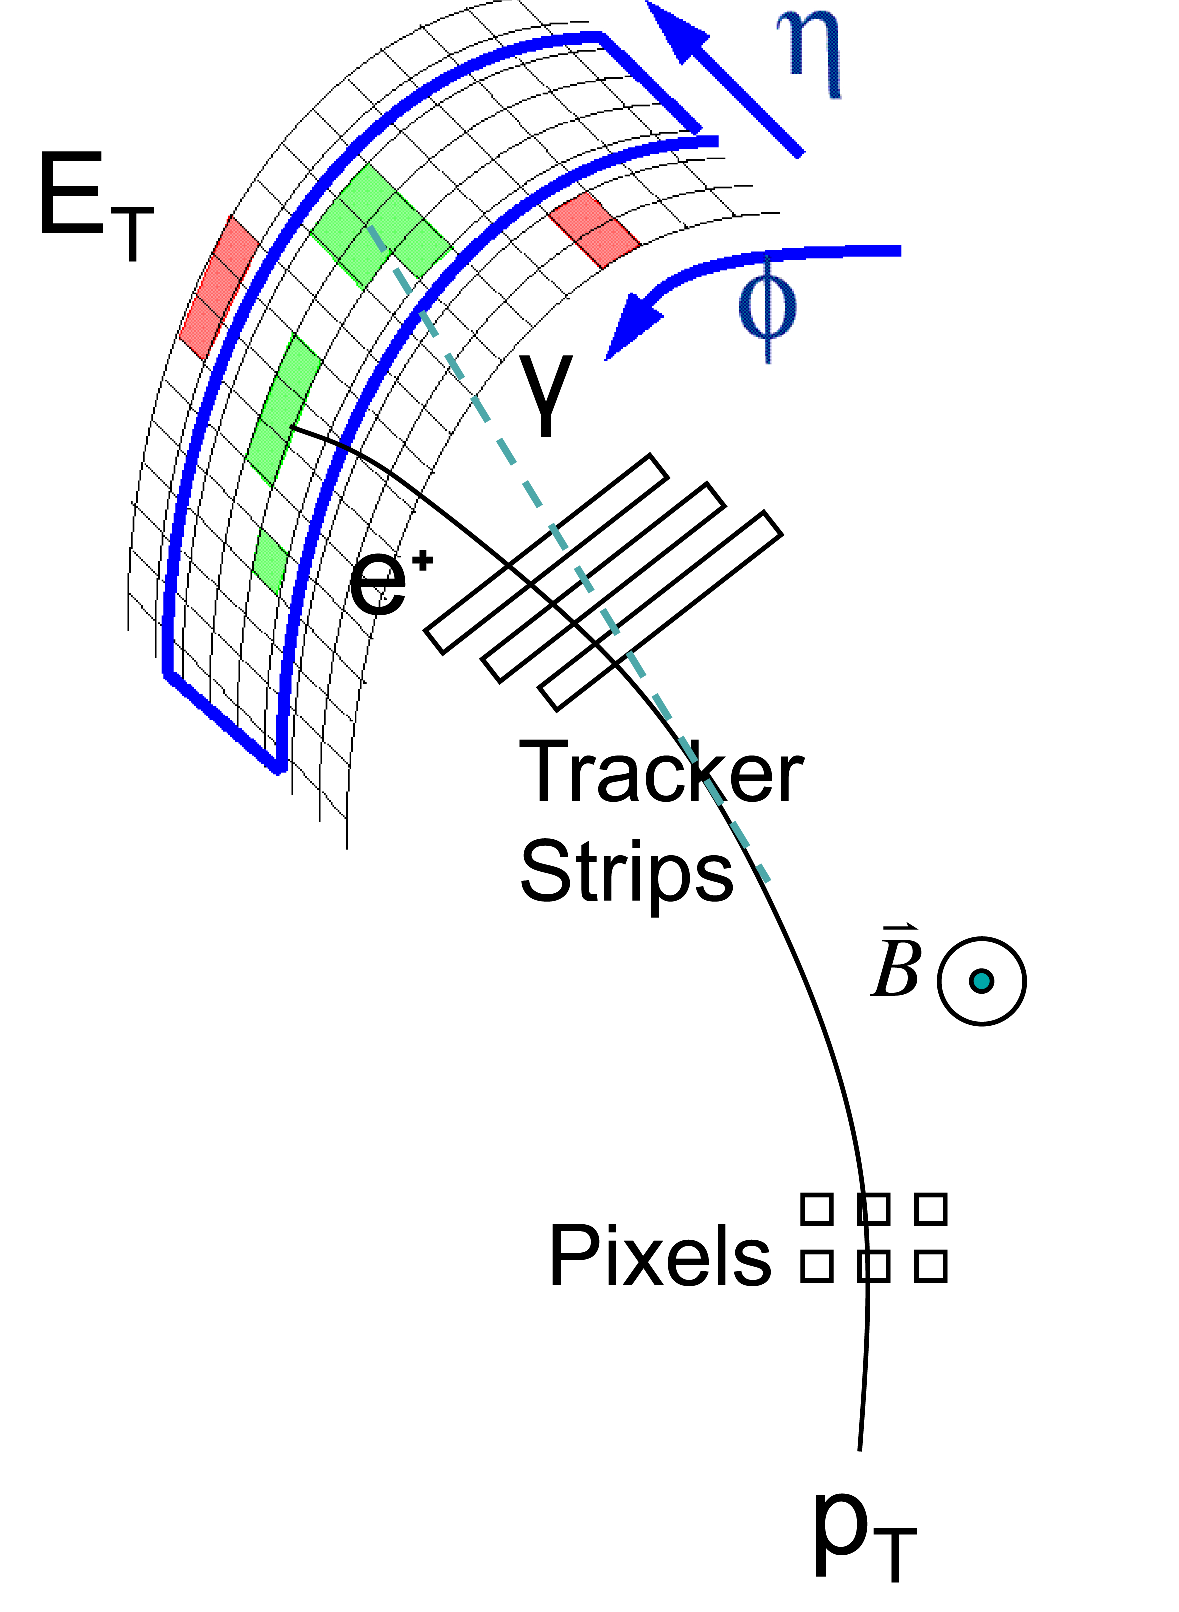
\includegraphics[width=0.40\textwidth]{eleReco}
\caption[Diagram of an electron and its signatures]{Diagram of an electron
travelling through the CMS detector. The electron emits bremsstrahlung radiation
as it bends, resulting in a signature in the ECAL consisting of both the
electron deposit and the radiated photon energies. The supercluster (blue) is a
collection of deposits which capture the electron and associated photon
energies.}
\label{fig:eleReco}
\end{figure}

Basic electron reconstruction can be done in one of two ways. An electron can
either be \emph{tracker-driven} or \emph{ECAL-driven}. The tracker-driven
approach is most effective for electrons that are low in $p_{T}$, starting 
with the collection of reconstructed tracks and searching for compatible hits in
the ECAL. The ECAL-driven approach, on the other hand, is designed to be more
efficient for the higher $p_{T}$ electrons, like those utilized in this
analysis. It begins with the supercluster collection and matches these to hits
in the inner tracker. The full electron trajectories are reproduced using a
Gaussian Sum Filter algorithm. This algorithm allows a more robust reconstruction
of the electron track when compared to the Kalman Filtering, as it is able to
account for the inherent kinks and bends due to the bremsstrahlung processes
the electron can undergo on its journey through the tracker~\cite{gsfElectrons}.

%loose reqs?

In this analysis, additional quality requirements are placed upon the electrons,
as outlined in Chapter~\ref{chapter:analysis}.

\section{Muon Reconstruction}
Muons in CMS are reconstructed using a combination of tracks, independently
reconstructed in the inner tracker and muon systems (colloquially referred to as
tracker tracks and standalone tracks, respectively. Like the electrons, muons
also have two possible modes of reconstruction, depending on whether the
matching begins from the tracker tracks or the standalone tracks.

\emph{Global muon} reconstruction begins in the muon system, taking the
standalone tracks and matching them to tracker tracks that follow a similar
propagation path. The global muon track is then built, using the hit information
in both systems. \emph{Tracker muon} reconstruction begins with tracker tracks
with $p_T > 0.5~GeV$ and total momenta $p > 2.5~GeV$. These tracks are then
treated as potential muons, and their expected paths are extended into the muon
system. If matching segments are found near to the extrapolated muon path, the
matching muon hits are added to the track hits in order to create the muon
object.

Although the inner tracker has greater resolving power in making track momenta
measurements, the muon system provides invaluable information for high $p_T$ ($\sim
100$ GeV) muons. Because these muons bend only slightly while traveling through
the tracker system, the additional hits in the muon system help to resolve the
momenta of these objects.

It is possible for tracks to be reconstructed in multiple muon candidates, as
more than one inner tracks can be geometrically close to the
backwards-extrapolated standalone tracks. These so-called `ghost' muons result
in a non-physical doubling of muon candidates. In order to treat this effect,
which becomes more pronounced in higher pile-up scenarios, the ghost muon pairs
are arbitrated. If two muons are nearby and share more than half of their
segments, the worse of the pair is discarded (as defined by a suite of
criteria based on the track quality measurements and, if needed, additional
identification criteria).

\section{Particle Flow}
Unique in CMS is the so-called \emph{particle flow} process, a suite of
reconstruction algorithms designed to fully reconstruct and identify all the
stable particles created in an event. More specifically, the algorithms are
designed to pick out all of the individual electrons, muons, charged hadrons,
neutral hadrons, and photons in an event. This information can be used in a
number of different ways, from using the identified objects themselves to
recombining the information into jets. Especially relevant to this analysis is
the particle flow muon criteria (which help to establish the collection of
well-identified muons used in the analysis) and the photon, charged hadron, and
neutral hadron collections, which are used to establish how much additional
energy is present near the candidate leptons.

Particle flow first lumps tracks, clusters, and muons into ``blocks,'' which are
simply groups of these objects which pass a loose connectedness test. Individual
particles are then combed out of each block. The process starts with muons,
identifying a particle-flow muon as a global muon with momenta compatible with a
tracker muon. The tracks, muons, and calorimeter signature attributed to the
found muons are then removed from the block and electrons are identified, using
criteria similar to those outline above. Again, associated tracks and
calorimeter clusters are removed from the block. Remaining calorimeter clusters
are assigned to (well-reconstructed) tracks if the deposits are consistent with
a charged-hadron hypothesis, or assigned to neutral hadron or photons, based on
whether the energy was deposited in the HCAL or ECAL. This procedure is
discussed in greater detail in \cite{pflow}.


%\section{Tau Reconstruction}
